\subsection{Interrelación Matrícula - Calificación Convocatoria}

   \begin{description}
      \item[Definición] En esta interrelación se deja constancia de que un
      alumno obtendrá una calificación de una determinada convocatoria de una
      asignatura en la que se encuentre matriculado.

      \begin{itemize}
       \item Una \textit{Matrícula} puede disponer de varios
             \textit{Calificación Convocatoria}.
       \item Una \textit{Calificación Convocatoria} solamente puede pertenecer a
             una \textit{Matrícula}.
      \end{itemize}

      \item[Características] La interrelación presenta las siguientes
                             características:

         \begin{itemize}
            \item \textbf{Nombre:} M-CC
            \item \textbf{Tipo de la interrelación:} El tipo de entidad
                  Calificación Convocatoria es débil por identificación respecto
                  al tipo de entidad Matrícula.
            \item \textbf{Cardinalidad de la interrelación:} 1:N
                  \begin{itemize}
                     \item Matrícula: dispone\_de (0,n)
                     \item Calificación Convocatoria: pertenece\_a (1,1)
                  \end{itemize}
            \item \textbf{Número de atributos:} Ninguno.
         \end{itemize}

      \item[Diagrama] La figura \ref{diagramaM-CC} muestra el diagrama de la
                      interrelación.

      \item \begin{figure}[!ht]
            \begin{center}
            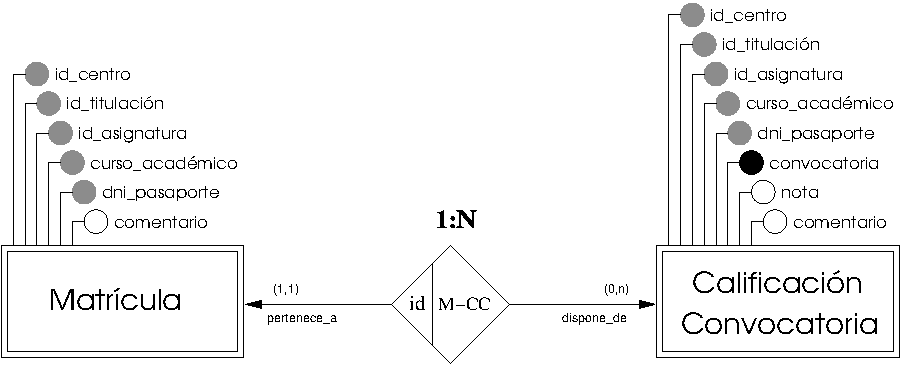
\includegraphics[]{07.Modelo_Entidad-Interrelacion/7.3.Analisis_Interrelaciones/diagramas/M-CC.pdf}
            \caption{Diagrama de la interrelación M-CC.}
            \label{diagramaM-CC}
            \end{center}
         \end{figure}

      \item[Ejemplo práctico del tipo de interrelación]

      \item \begin{center}
            \begin{tabular}{ | r r | }
            \hline
            \multicolumn{2}{ | c | }{\textbf{Tipo de interrelación M-CC}} \\
            \hline
            \textbf{Matrícula} & \\
            id\_centro & 15 \\
            id\_titulación & 3\\
            id\_asignatura & 17\\
            curso\_académico & 2008 \\
            dni\_pasaporte & 01234567A \\
            \hline
            \textbf{Calificación Convocatoria} & \\
            id\_centro & 15 \\
            id\_titulación & 3\\
            id\_asignatura & 17\\
            curso\_académico & 2008 \\
            dni\_pasaporte & 01234567A \\
            convocatoria & febrero \\
            nota & 8,4 \\
            \hline
            \end{tabular}
         \end{center}
   \end{description}
